\documentclass[11pt, oneside]{article}   	% use "amsart" instead of "article" for AMSLaTeX format
\usepackage{geometry}                		% See geometry.pdf to learn the layout options. There are lots.
\geometry{letterpaper}                   		% ... or a4paper or a5paper or ... 
\usepackage{graphicx}				% Use pdf, png, jpg, or eps§ with pdflatex; use eps in DVI mode
								% TeX will automatically convert eps --> pdf in pdflatex		
\usepackage{amssymb}
\usepackage{amsmath}
\usepackage{parskip}
\usepackage{color}
\usepackage{hyperref}

\graphicspath{{/Users/telliott_admin/Tex/png/}}
% \begin{center} 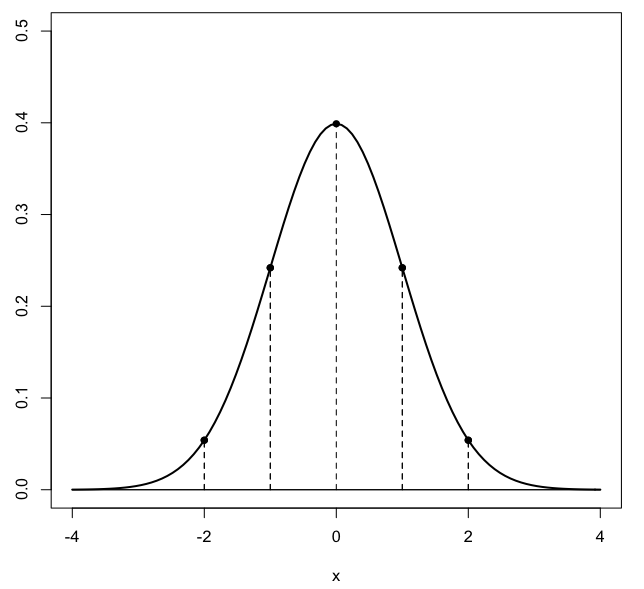
\includegraphics [scale=0.4] {gauss3.png} \end{center}

%break
\title{Surface integrals}
\date{}

\begin{document}
\maketitle
\Large
Here we consider some basic facts about surface integrals. 

For a point on a surface, we use the tangent plane approximation.  Imagine that the surface is tiled, composed of numerous tiny planes.  At any point, the surface is locally flat, having uniform slope.  

We will need to find the angle $\theta$ this plane makes with the horizontal.  We use that angle for this calculation:

\[ dA = \cos \theta \ dS \]
\[ dS = \frac{1}{\cos \theta} \ dA \]

A little piece of area on the surface is made smaller in its projection to the $xy$-plane by this factor.

Like any plane, we describe a tangent plane by its normal vector, $\mathbf{n}$.  
\begin{center} 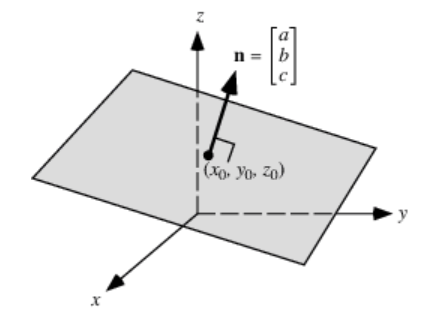
\includegraphics [scale=0.4] {normal_vector.png} \end{center}

Can you see that $\mathbf{n}$ makes the same angle $\theta$ with the $z$-axis or $\hat{\mathbf{k}}$ unit vector as the surface element makes with the $x,y$-plane, so that
\begin{center} 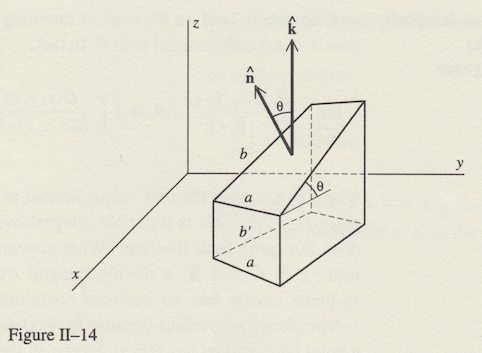
\includegraphics [scale=0.3] {tilt.png} \end{center}

\[ \mathbf{n} \cdot \hat{\mathbf{k}} = |\mathbf{n}| |\hat{\mathbf{k}}| \ \cos \theta \]

Since $\hat{\mathbf{k}}$ is a unit vector, $|\hat{\mathbf{k}}| = 1$

\[ \mathbf{n} \cdot \hat{\mathbf{k}} = |\mathbf{n}| \ \cos \theta \]
\[ \cos \theta = \frac{\mathbf{n} \cdot \hat{\mathbf{k}} }{|\mathbf{n}|} \]

As always, find $\mathbf{n}$ by first finding two vectors in the plane and then forming the cross-product.  

We will use the basis vectors $( \hat{\mathbf{i}}, \hat{\mathbf{j}}, \hat{\mathbf{k}} )$, so think about a cross-section of the plane at the point of interest, parallel to the $xz$-plane.  

The cross-section of the surface is just a line with some slope to it, $f_x$.  For each unit of change in the $x$ or $\hat{\mathbf{i}}$ direction, there is a change of $f_x$ in the $\hat{\mathbf{k}}$ direction and none in the $\hat{\mathbf{j}}$ direction.  

\begin{center} 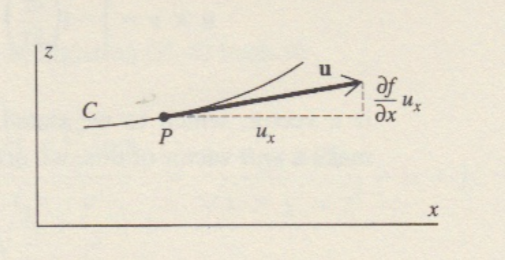
\includegraphics [scale=0.5] {ux.png} \end{center}

So one vector in the plane is
\[ \langle 1, 0, f_x \rangle \]

By symmetry, the second is
\[ \langle 0, 1, f_y \rangle \]

The cross-product is evaluated by forming the matrix

\[
\begin{bmatrix} 
  \hat{\mathbf{i}}  & \hat{\mathbf{j}}  &  \hat{\mathbf{k}} \\ 
  1  &  0 & f_x \\
  0  &  1 & f_y
\end{bmatrix}
\]

and evaluating its "determinant"

\[  \mathbf{n} = \langle -f_x, -f_y, 1 \rangle   \]

According to this formulation $\mathbf{n} \cdot \hat{\mathbf{k}}$ is $1$!  

Returning to what we wrote above
\[ \cos \theta = \frac{\mathbf{n} \cdot \hat{\mathbf{k}} }{|\mathbf{n}|} = \frac{1}{|\mathbf{n}|} \]

Our currency exchange rate for area in the plane compared to area on the sloped tangent plane is 
just
\[ dS = \frac{1}{\cos \theta} \ dA \]
\[ dS = |\mathbf{n}| \ dA \]

and
\[ |\mathbf{n}| = \sqrt{1 + f_x^2 + f_y^2} \]

Hence 
\[ \iint_S \ dS = \iint \sqrt{1 + f_x^2 + f_y^2} \ dx \ dy \]

\subsection*{aid to memory}
One way to help remembering this formula is by analogy to line integrals, which seem pretty straightforward to set up, though they are often an arithmetic mess.

The small element of the path is $ds$ so by Pythagoras we get 
\[ ds^2 = dx^2 + dy^2 \] 
and then a little rearrangement gives:
\[ ds^2 = \ [ \ 1 + (\frac{dy}{dx})^2 \ ] \ dx^2 \] 
\[ ds = \ [ \ \sqrt{1 + y'^2} \ ] \ dx \]

The area element for surfaces is almost exactly the same:
\[ dS =  \sqrt{1 + f_x^2 + f_y^2} \  \cdot \ dA \]

So let's just remember the surface area element $dS$ as an extension of $ds$ to 2 dimensions.

\subsection*{plane}
Consider the plane that cuts through each axis at its unit dimension:  i.e. $P = (1,0,0)$, $Q = (0,1,0)$, and $R = (0,0,1)$.  Purely from symmetry, we could argue that the normal vector should be 
\[ \mathbf{N} = \langle 1,1,1 \rangle \]

By the same argument, the equation of the plane should be 
\[ x + y + z = c = 1 \]
where we evaluate the constant $c = 0$ from looking at the diagram.

\begin{center} 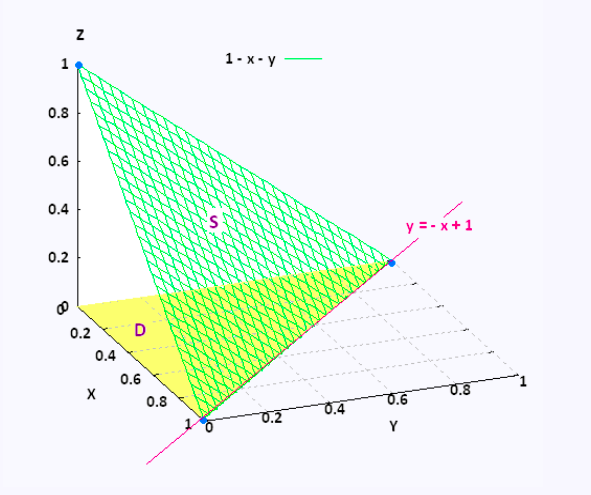
\includegraphics [scale=0.5] {plane_surface.png} \end{center}

Alternatively, obtain two vectors in the plane by subtraction:
\[ \mathbf{u} = PQ = \langle 1,-1,0 \rangle \]
\[ \mathbf{v} = PR = \langle 1,0,-1 \rangle \]
\[ \mathbf{u} \times \mathbf{v} = \langle -1, -1, -1 \rangle \]
which is what we had, within sign.  So we will say that 
\[ \mathbf{\hat{n}} = \frac{1}{\sqrt{3}} \langle 1, 1, 1 \rangle \]

We can get the Jacobian $J$ in two ways.  First
\[ x + y + z = 1 \]
\[ z = 1 - x - y \]
\[ f_z = -1 \]
\[ f_y = -1 \]
\[ J = \sqrt{f_x^2 + f_y^2 + 1} = \sqrt{3} \]

Alternatively
\[ | \mathbf{u} \times \mathbf{v} | = | \langle -1, -1, -1 \rangle | = \sqrt{3} \]
Either way, the area element on the surface is
\[ dS = J \ dA = \sqrt{3} \ dA \]

The other issue is the bounds for the shadow in the $xy$-plane.  We can see that the slope of the line relating $x$ and $y$ is $-1$ and the $y$-intercept is $1$ so
\[ y = 1 - x \]

Now just set up the double integral
\[ \iint_R J \ dA = J \int_0^1 \int_0^{1-x} \ dy \ dx \]
The inner integral is
\[ 1 - x \]
So the outer integral is
\[ \sqrt{3} \int_0^1 1 - x \ dx \]
\[ \sqrt{3} \ [ \ x - \frac{x^2}{2} \ \bigg |_0^1 \ ] \ = \frac{\sqrt{3}}{2} \]

We check this as follows. The lengths of the three sides of the surface we're measuring are each
\[ | \mathbf{u} | = | \langle 1,-1,0 \rangle | = \sqrt{2}  \]

The point midway along the base to which we would draw an altitude from $R$ is $(1/2,1/2,0)$ so its distance from $R$ is
\[ \sqrt{(\frac{1}{2})^2 + (\frac{1}{2})^2  + (-1)^2 } = \sqrt{\frac{3}{2}} \]
The area of the triangle is
\[ \frac{1}{2} \sqrt{2} \ \sqrt{\frac{3}{2}} = \frac{\sqrt{3}}{2} \]

Note:  we had the length of the normal vector as $\sqrt{3}$.  This is the rate of exchange $J$ between the surface area and the area of the projection in the plane.  That projection is just a triangle of area $1/2$, hence the final answer is $\sqrt{3}/2$.

\subsection*{volume}

As long as we're here, let's do the volume:
\[ V = \iint_R z \ dy \ dx \]
\[ = \int_0^1 \int_0^{1-x} (1 - x - y) \ dy \ dx \]
No Jacobian here!

The inner integral is
\[ y - xy - \frac{y^2}{2} \ \bigg |_0^{1-x} \]
\[ = 1 - x - (x - x^2) - \frac{1}{2} (1 - 2x + x^2) \]
\[ = \frac{x^2}{2} - x + \frac{1}{2} \]

The outer integral is
\[ \frac{x^3}{6} - \frac{x^2}{2} + \frac{x}{2} \ \bigg |_0^1 = \frac{1}{6} \]

In solid geometry, we had that
\[ V = \frac{1}{3} \ \text{base} \times \text{height} \]
which matches.
 
\subsection*{sphere}
Our formula for the surface area element is
\[ dS =  \sqrt{1 + f_x^2 + f_y^2} \  \cdot \ dA \]

With just this formula we can also calculate the surface area of a sphere.  Write
\[ x^2 + y^2 + z^2 = a^2 \]
where $a$ is the constant radius.  Then
\[ z = f(x,y) = \sqrt{a^2 - x^2 - y^2} \]
\[ f_x = \frac{1}{2} \ \frac{-2x}{\sqrt{a^2 - x^2 - y^2}} = -\frac{x}{z} \]
or by implicit differentiation:
\[ z^2 = a^2 - x^2 - y^2 \]
\[ 2 z \ dz = - 2 x \ dx \]
and then we get the same thing as before.  Similarly $f_y = -y/z$.

Now use the formula.  Plugging in $f_x$ and $f_y$:
\[ dS = \ [ \ \sqrt{(\frac{x}{z})^2 + (\frac{y}{z})^2 + 1} \  ] \ dA \]
\[ = \frac{1}{z}  \ [ \ \sqrt{(x^2 + y^2 + z^2} \  ] \ dA \]
\[ dS = \frac{a}{z} \ dA \]

We want to set up $\int dS$, although it's pretty ugly in $x,y$.  We get
\[ \int_{-a}^a \int_{-\sqrt{a^2-x^2}}^{\sqrt{a^2-x^2}} \frac{a}{\sqrt{a^2 - x^2 -y^2}} \ dy \ dx \]
The inner integral is essentially:
\[ \int \frac{1}{\sqrt{c^2 -y^2}} \ dy \]
where $c^2 = a^2 - x^2$.  We don't have $y$ so we need to do a trig substitution.  This comes out to be
\[ \sin^{-1} \frac{y}{c} \]
evaluated between $-c$ and $c$.  
\[ \sin^{-1} \frac{y}{c} \  \bigg |_{-c}^c = \frac{\pi}{2} - (- \frac{\pi}{2}) = \pi  \]
The outer integral is then
\[ \int_{-a}^a \pi a \ dx = 2 \pi a^2 \]

It is much nicer to switch to $r,\theta$.  We do this to check ourselves. Let
\[ x^2 + y^2 = r^2 \]
\[ z^2 = a^2 - x^2 - y^2 = a^2 - r^2 \]
\[ \iint dS = \frac{a}{z} \ r \ dr \ d \theta \]
\[ = \int_0^{2 \pi} \int_0^a  \frac{a}{\sqrt{a^2 - r^2}} \ r \ dr \ d \theta \]
That extra factor of $r$ from the surface area element (or the Jacobian, if you like), makes everything easy.

The inner integral is essentially $1/\sqrt{u} \ du$
\[ \int \frac{1}{\sqrt{a^2 - r^2}} \ r \ dr = -\sqrt{a^2 - r^2}  \]
so we obtain
\[ a \ [ \ -\sqrt{a^2 - r^2} \ ] \ \bigg |_0^a = a^2 \]
which is zero at the upper bound and $-a^2$ at the lower bound.  Subtracting, we obtain $a^2$, and with the outer integral, the whole thing is $2 \pi a^2$.

We are a factor of $2$ off from the known result using both methods, and realize that when we wrote 
\[ z = f(x,y) = \sqrt{a^2 - x^2 - y^2} \]
we were only looking at the upper hemisphere, so we have found the missing factor of $2$.  The result above is for the hemisphere.

\subsection*{Paraboloid}
Our purpose here is to develop two simple examples, the surface areas of the paraboloid and the hemisphere.  For the paraboloid, consider one which has its vertex at $z=1$ and opens down
\[ z = 1 - x^2 - y^2 \]
When $z=0$ this is just $x^2 + y^2 = 1$.  We find that 
\[ f_x = -2x \]
\[ f_y = -2y \]
\[ \sqrt{f_x^2  + f_y^2 + 1} = \sqrt{4x^2 + 4y^2 + 1} \]
This would be a good time to switch to polar coordinates.
\[ x^2 + y^2 = r^2 \]
\[ \sqrt{(f_x)^2 + (f_y)^2 + 1} = \sqrt{4r^2 + 1} \]
 So we have the integral
\[ \int \int \sqrt{4r^2 + 1} \ \ r \ dr \ d \theta \]
with the $r$ term coming from the usual source. 
The inner integral is
\[ \frac{1}{12} \  (4r^2 + 1)^{3/2} \]
For the unit circle ($r=0 \rightarrow 1$), and multiplying by $2\pi$ for the outer integral, this is
\[ 2 \pi \ \frac{1}{12} \ [ \  (5)^{3/2} - 1^{3/2} ] = \frac{\pi}{6} \ [ \ 5 \sqrt{5} - 1 \ ] \]
In general, if the limits for the radius are $r=a \rightarrow r=b$ we will have
\[ \frac{\pi}{6}\ [ \ (4b^2 + 1)^{3/2} - (4a^2 + 1)^{3/2} \ ] \]

We can check this using the surface of a solid of revolution.  Turn the function to have more familiar variables.  It is $y=\sqrt{x}$.  Rotated around the $x$-axis, this solid has a cross-section at each point with circumference $2 \pi y = 2 \pi \sqrt{x}$.  The surface area is
\[ \int 2 \pi \sqrt{x} \ ds \]
The surface area element is 
\[ ds = \sqrt{1 + f'(x)^2} \ dx \]
(Looks familiar!)  So $f'(x)^2 = \frac{1}{4x}$ and we have
\[ \int 2 \pi \sqrt{x} \ \sqrt{1 + \frac{1}{4} x} \ dx \]
\[ 2 \pi \int \sqrt{x + \frac{1}{4}} \ dx \]
\[ \frac{4}{3} \pi \ (x + \frac{1}{4})^{3/2} \]
\[ \frac{\pi }{6} \ (4x + 1)^{3/2} \]
evaluated between $x=0 \rightarrow 1$, we obtain
\[ \frac{\pi }{6} \ [ \ (5)^{3/2} - 1^{3/2} \ ] \ = \frac{\pi}{6} \ [ \ 5 \sqrt{5} - 1 \ ] \]
which matches what we had by the new method.

\subsection*{vector field}
To finish up, let's go back to

\[ \iint_S \mathbf{F} \cdot \hat{\mathbf{n}} \ dS \]

in $x,y$-coordinates, this is

\[ \hat{\mathbf{n}} \ dS = < -f_x,-f_y,1>  \ dx \ dy \]

How do we get this?  Above we derived an expression for the surface element $dS$

\[ dS = \ \sqrt{f_x^2 + f_y^2 + a} \ dx \ dy \]

so in $R$ the integral becomes

\[ \iint_R \mathbf{F} \cdot \hat{\mathbf{n}} \ \sqrt{1 + f_x^2 + f_y^2} \ dx \ dy \]

Recall from earlier that

\[  \hat{\mathbf{n}} = \frac{\mathbf{u} \times \mathbf{v}}{| \mathbf{u} \times \mathbf{v} |} = \frac{1}{\sqrt{f_x^2  + f_y^2 + 1}} \ < -f_x, - f_y , 1 > \]

The square root cancels, leaving us with

\[ \iint_R \mathbf{F} \cdot \ < -f_x,-f_y,1>  \ dx \ dy \]

\subsection*{example}

Suppose that
\[ \mathbf{F} = z \hat{\mathbf{i}} - y \hat{\mathbf{j}} + x  \hat{\mathbf{k}} \]
\[ \mathbf{F} = \ <z,-y,x> \]
and $S$ is the part of the plane $x + 2y + 2z = 2$ in the positive octant, crossing through the points $(2,0,0),(0,1,0)$ and $(0,0,1)$.

Rearrange the equation of the surface
\[ f(x,y) = z = 1 - \frac{x}{2} - y \]
\[ f_x = -\frac{1}{2} \]
\[ f_y = -1 \]

We want to compute
\[ \iint_R \mathbf{F} \cdot \ < -f_x,-f_y,1>  \ dx \ dy \]

Plugging in
\[ \mathbf{F} \cdot \ < -f_x,-f_y,1> \]
\[ = \ <z,-y,x> \ \cdot \ < \frac{1}{2},1,1> \]
\[ = \frac{1}{2}(1 - \frac{x}{2} - y) - y + x \]
\[ = \frac{1}{2} + \frac{3}{4}x - \frac{3}{2}y \]
So the integral is
\[ =  \iint_R \ \frac{1}{2} + \frac{3}{4}x - \frac{3}{2}y  \ dx \ dy \]

If we integrate with respect to $dy$ first, using $y = 0 \rightarrow y = -x/2 + 1$, the inner integral is
\[ = \frac{1}{2} y + \frac{3}{4}xy - \frac{3}{4} y^2 \  \bigg |_{y=0}^{y = -x/2 + 1} \]
\[ = \frac{1}{2}(-\frac{x}{2} + 1) + \frac{3}{4}x(-\frac{x}{2} + 1) -  \frac{3}{4}(-\frac{x}{2} + 1)^2 \]
Now
\[ (-\frac{x}{2} + 1)^2 = \frac{x}{4} -x + 1\]
 so we have
 \[ = \frac{1}{2}(-\frac{x}{2} + 1) + \frac{3}{4}x(-\frac{x}{2} + 1) -  \frac{3}{4}(\frac{x}{4} -x + 1) \]
\[ = -\frac{x}{4} + \frac{1}{2} - \frac{3}{8}x^2 + \frac{3}{4}x - \frac{3}{16}x + \frac{3}{4}x - \frac{3}{4} \]
\[ = - \frac{1}{4} -\frac{x}{4} - \frac{3}{8}x^2 + \frac{3}{4}x - \frac{3}{16}x + \frac{3}{4}x \]
\[ = - \frac{1}{4} +\frac{5}{4}x  - \frac{3}{16}x - \frac{3}{8}x^2  \]
\[ = - \frac{1}{4} + \frac{17}{16}x  - \frac{3}{8}x^2 \  \]
and then the inner integral is
\[ = - \frac{1}{4}x + \frac{17}{32}x^2  - \frac{1}{8}x^3 \  \bigg |_0^1 = \frac{5}{32}  \]
The answer given is $1/2$ so I suppose there is a mistake somewhere..
\subsection*{example 2}

Take the surface of the unit sphere ($z = \sqrt{1-x^2-y^2}$ in the positive octant.  The region $R$ in the $xy$-plane is the unit circle in that quadrant.

We find $f_x = -x/z$ and $f_y = -y/z$ as usual and 
\[ \mathbf{F} = xz \hat{\mathbf{i}} + z^2 \hat{\mathbf{k}} \]
\[ \mathbf{F} = \ <xz,0,z^2> \]
So 
\[ \mathbf{F} \cdot \ < -f_x,-f_y,1> \]
\[ = \ <xz,0,z^2> \ \cdot \ < \frac{x}{z},\frac{y}{z},1> \]
\[ = x^2 + z^2 \]
\[ = x^2 + 1 - x^2 - y^2 \]
We want compute
\[ = \iint_R 1 -y^2 \ dx \ dy \]

The first part of this integral is just the area of the quarter circle of radius $1$, equal to $\pi/4$.
For the second term, we want to integrate over the same region, which suggests the use of polar coordinates 
\[ x = r \cos \theta \]
\[ y = r \sin \theta \]
\[ \iint_R y^2 \ dx \ dy \]
\[ = \int_0^{\pi/2} \int_0^1 r^2 \sin^2 \theta \ r \ dr \ d \theta \]

If we do $r^3 dr$ first we get a factor of $1/4$ so we have 
\[ \frac{1}{4} \int_0^{\pi/2} \sin^2 \theta \ d \theta \]
\[ = \frac{1}{4} \frac{1}{2}(\theta - \frac{1}{2}\sin 2 \theta) \  \bigg |_0^{\pi/2}  \]
\[ = \frac{1}{8} (\frac{\pi}{2}) \]
Combining with $\pi/4$ (and remembering the minus sign)
\[ = \frac{\pi}{4} - \frac{\pi}{16} = \frac{3}{16} \pi \]

\end{document}